\documentclass[a4paper,12pt]{report} %togliere quadre per ridurre pagine
\usepackage{graphicx}
\usepackage{hyperref}
\usepackage{placeins}
\usepackage{float}
\usepackage[acronym,nomain,nonumberlist]{glossaries}

\usepackage{titlesec}
\usepackage{enumerate}
\setcounter{tocdepth}{4}
\setcounter{secnumdepth}{4}

\makeatletter
\renewcommand{\thesection}{%
  \ifnum\c@chapter<1 \@arabic\c@section
  \else \thechapter.\@arabic\c@section
  \fi
  \let\Hy@linktoc\Hy@linktoc@none
}
\makeatother

\usepackage{fancyhdr}
\pagestyle{fancy}
\lhead{Marco Rossanese} % controls the left corner of the header
\chead{} % controls the center of the header
\rhead{\rightmark} % controls the right corner of the header
\lfoot{5G Systems} % controls the left corner of the footer
\cfoot{} % controls the center of the footer
\rfoot{Page~\thepage} % controls the right corner of the footer
\renewcommand{\headrulewidth}{0.4pt}
\renewcommand{\footrulewidth}{0.4pt}


\makeglossaries


\begin{document}
\pagenumbering{gobble}
\clearpage\pagestyle{empty}

\title{

\includegraphics[width=0.4\textwidth]{pics/unipd.jpg}~\\[1.5cm]
NETWORK SLICING OVERVIEW
\\
}

\author{Marco Rossanese 1177738
\\5G Systems - Prof. Stefano Tomasin
\\marco.rossanese@studenti.unipd.it~\\[1cm]
\includegraphics[width=0.4\textwidth]{pics/dei.jpg}
}

\maketitle
\newpage


\tableofcontents
\newpage
\printglossaries
\newpage
%%%%%%%%%%%%%%%%%%%%%%%%%%%%%%%%%%%%%%%%%%%%%%%%%%%%%%%%%%%%%%%%%%%%%%%%%%%%%%%%%%%%%%%%%

% Acronym definitions
\newacronym{sdn}{SDN}{Software Defined Network}
\newacronym{mno}{MNO}{Mobile Network Operators}
\newacronym{ngmn}{NGMN}{Next Generation Mobile Networks}
\newacronym{sil}{SIL}{Service Instance Layer}
\newacronym{nsil}{NSIL}{Network Service Instance Layer}
\newacronym{e2e}{E2E}{End to End}
\newacronym{e2e}{E2E}{End to End}
\newacronym{fh}{FH}{Fronthaul}
\newacronym{bh}{BH}{Backthaul}
\newacronym{CN}{CN}{Core Network}
\newacronym{vi}{VI}{Virtual Infrastructure}
\newacronym{IaaS}{IaaS}{Infrastructure-as-a-Service}
\newacronym{NS}{NS}{Network Services}
\newacronym{VNF}{VNF}{Virtual Network Functions}
\newacronym{MANO}{MANO}{Management and Orchestration}
\newacronym{NBI}{NBI}{Northbound Interface}
\newacronym{SBI}{SBI}{Southbound Interface}
\newacronym{MTA}{MTA}{Multi-Tenancy Application}
\newacronym{NF}{NF}{Network Functions}
\newacronym{CP}{CP}{Control Plane}
\newacronym{UP}{UP}{User Plane}
\newacronym{AN}{AN}{Access Network}
\newacronym{RAT}{RAT}{Radio Access Technology}
\newacronym{NFV}{NFV}{Network Functions Virtualization}
\newacronym{eMBB}{eMBB}{enhanced Mobile Broadband}
\newacronym{mMTC}{mMTC}{massive Machine Type Communications}
\newacronym{URLLC}{URLLC}{Ultra‐Reliable Low‐Latency Communications}
\newacronym{VM}{VM}{Virtual Machines}
\newacronym{InP}{InP}{Infrastructure provider}
\newacronym{ONF}{ONF}{Open Networking Foundation}
\newacronym{SLA}{SLA}{Service Level Agreements}
\newacronym{KPI}{KPI}{Key Performance Indicators}
\newacronym{NFVI}{NFVI}{Network Functions Virtualization Infrastructure}
\newacronym{VIM}{VIM}{Virtual Infrastructure Manager}
\newacronym{VNFM}{VNFM}{Virtual Network Function Manager}
\newacronym{RO}{RO}{Resource Orchestrator}
\newacronym{NSO}{NSO}{Network Service Orchestrator}
\newacronym{NMS}{NMS}{Network Management System}
\newacronym{OSS/BSS}{OSS/BSS}{Operation/Business Support System}
\newacronym{EM}{EM}{Element Management}
\newacronym{IC}{IC}{Infrastructure SDN controller}
\newacronym{TC}{TC}{Tenant SDN controller}
\newacronym{EPC}{EPC}{Evolved Packet Core}
\newacronym{RAN}{RAN}{Radio Access Network}
\newacronym{QoS}{QoS}{Quality of Service}
\newacronym{QoE}{QoE}{Quality of Experience}
\newacronym{RRM}{RRM}{Radio Resource Management}
\newacronym{HSS}{HSS}{Home Subscriber System}
\newacronym{UDM}{UDM}{Unified Data Management}
\newacronym{AUSF}{AUSF}{Authentication Server Functions}
\newacronym{IoT}{IoT}{Internet of Things}
\newacronym{UPF}{UPF}{User Plane Processing Functions}
\newacronym{CPF}{CPF}{Control Plane Processing Functions}
\newacronym{AMF}{AMF}{Access and Mobility Management Function}
\newacronym{SMF}{SMF}{Session Management Function}
\newacronym{UDM}{UDM}{Unified Data Management}
\newacronym{NAS}{NAS}{Non‐Access Stratum}
\newacronym{RRC}{RRC}{Radio Resource Control}
\newacronym{RLC}{RLC}{Radio Link Control}
\newacronym{PDCP}{PDCP}{Packet Data Convergence Protocol}
\newacronym{API}{API}{Application Program Interface}
\newacronym{PCF}{PCF}{Policy Control Function}
\newacronym{NEF}{NEF}{Network Exposure Function}
\newacronym{NRF}{NRF}{NF Repository Function}
\newacronym{N3IWF}{N3IWF}{Non-3GPP InterWorking Function}
\newacronym{UDR}{UDR}{Unified Data Repository}
\newacronym{NSSF}{NSSF}{Network Slice Selection Function}
\newacronym{AF}{AF}{Application Function}
\newacronym{CSMF}{CSMF}{Communication Service Management Function}
\newacronym{NSMF}{NSMF}{Network Slice Management Function}


%%%%%%%%%%%%%%%%%%%%%%%%%%%%%%%%%%%%%%%%%%%%%%%%%%%%%%%%%%%%%%%%%%%%%%%%%%%%%%%%%%%%%%%%%%%

\newpage
\pagenumbering{arabic}
\setcounter{page}{1}
\pagestyle{fancy}
\section{Introduction}
Mobile networks are a fundamental topic for modern society because they guarantee communications and access
to information on a tap of our fingers. Furthermore we expect that the data flowing per month will be around 50 exabytes and this is caused mainly by video services.
Indeed in the last years, mobile operators are moving from a voice-oriented infrastructures to
data-oriented ones and they are not able to keep pace with the calculated traffic volume. Facing such new problems, operators have
invested a lot in research efforts toward the designing of the Fifth Generation mobile architecture, in order to provide innovative solutions for new capabilities and revenue sources. Network slicing is one of proposed innovation to push forward the frontier of mobile communications and it will discussed in this overview.\\
5G Network slicing allows \gls{mno} to share
physical infrastructures they have to the simultaneous deployment
of multiple independent logical networks, managed with respect
to their specific service requirements. 
%The availability of this vertical market\footnote{A vertical market is a group of companies that serve each other's specialized needs and do not serve a broader market, therefore it is mostly focused on meeting the needs of one specific industry.} multiplies
%the money incoming opportunities of the network infrastructure as new
%opportunities come into play (e.g., automotive industry, e-health) and an higher
%infrastructure capacity utilization can be achieved by letting network slice
%requests and exploiting multiplexing gains.\\
For example, different services like automotive, tactile internet or massive IoT can be put in practice by exploiting different network slice
instances, that is a set of virtual network functions
that run on the same infrastructure with customized policies. Thanks to that,
heterogeneous requirements can run on the same infrastructure, since
different instances can be orchestrated and set independently
according to the specifics requested. Furthermore, this is executed in a
costly efficient way because as the a network slice shares the same
physical infrastructure with different slices.\\
A network slice is defined by \gls{ngmn} as “\textit{a set of network functions, and
resources to run these network functions, forming a complete instantiated
logical network to meet certain network characteristics required by the Service
Instance(s)}”.\\
According to NGMN, the concept of network slicing is ideally composed by: the \gls{sil} that involves the business/end user services provided by operators or by the party which leases the services by the operators; the \gls{nsil} is set of functions to run the instances and the resource layer, which consists of the
resources such as compute, network, memory, storage.\\
The target of slicing is to realize
\gls{e2e} network slices from the mobile edge,
through the mobile transport (\gls{fh}/\gls{bh}) and up until
\gls{CN}.\\
The two main tools needed to allow different degrees
of control and automation in NSIL and resource layers are: the \gls{vi} under the control and operation
of different tenants in agreement with an \gls{IaaS} model\footnote{Form of cloud computing providing computed and virtualized resources over the internet} to split information from used hardware; \gls{NS} owned by tenants, that is actually creation of a service instance.
The VIs can be operated by \gls{sdn}, NS are instantiated directly over a shared infrastructure
and as a set of \gls{VNF} connected through
one or more VNF forwarding graphs are necessary to define the life cycle of the slice; both of them will be discussed later.\\
Multi-tenancy is an characteristic that must be achieved to guarantee separation, isolation, and independence between
different slices decoupled from the shared underlying resources.\\
\begin{figure}[H]
\centering
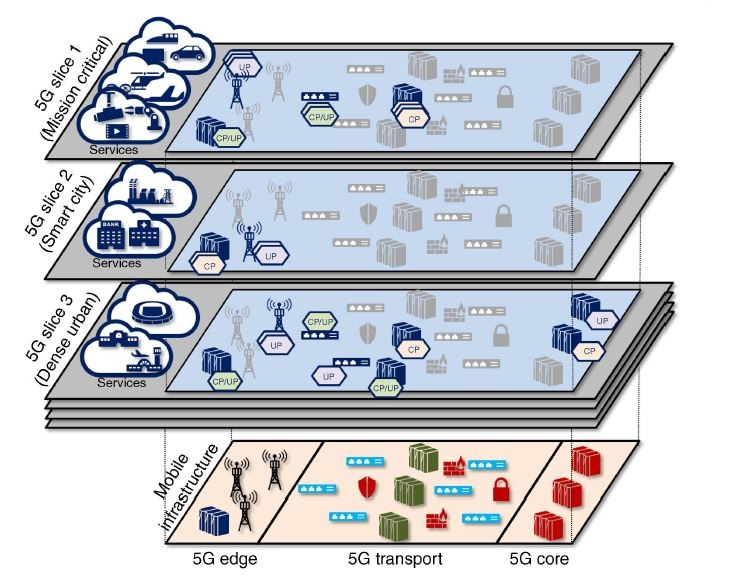
\includegraphics[scale=0.65]{pics/1.JPG}
\caption{Example of network slicing in 5G. \cite{al20185g}}
\label{layers}
\end{figure}
After this general overview this essay will treat accurately all the necessary fundamental components in order to fully understand how 5G network slicing is planned actually to be built. \cite{al20185g} \cite{marsch20185g}


\newpage
\section{Structural components} 
Starting from how an architecture for network slicing is conceptually made, it will be explained what it should achieve and involve, that is, the aspects of modularization, resource virtualization, virtual infrastructure and NS management; they will be the main topics of this section.
\begin{figure}[h]
\centering
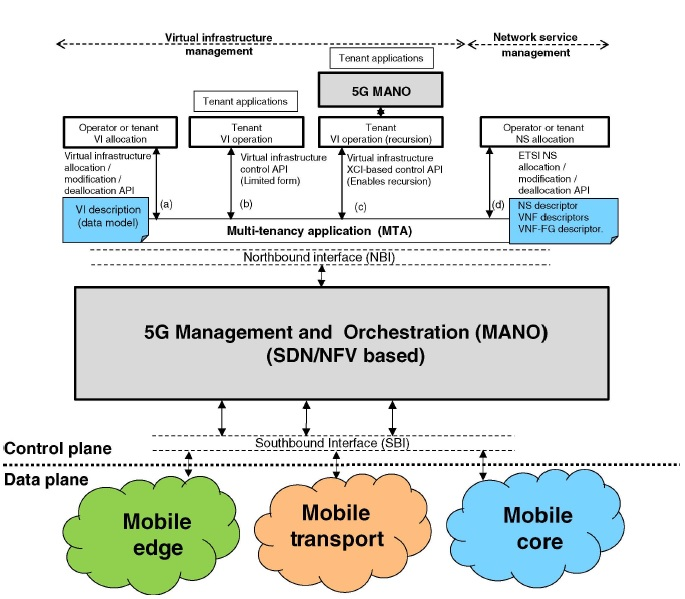
\includegraphics[scale=0.67]{pics/2.JPG}
\caption{Architecture for network slicing. \cite{al20185g}} 
\label{Arch}
\end{figure}
As anticipated about virtualization of the infrastructure, the SDN design is proposed in Fig. \ref{Arch} and follows the principles of:
\begin{itemize}
\item data and control plane fully decoupled;
\end{itemize}
\begin{itemize}
\item control logically centralized;
\end{itemize}
\begin{itemize}
\item applications having an abstracted view of resources and states.
\end{itemize}
The data plane is actually the resource layer where mobile edge, mobile transport, and core are present. The infrastructure is made of links, forwarding nodes like a router or a switch, cloud nodes  and a set of network, computing and storage resources.\\
The control plane is divided into two layers: an application layer at the top and at the bottom the \gls{MANO}. \\
The design of the MANO is based on the ETSI management and orchestration of the network by means of a framework exploiting SDN-based control. The MANO
provides a panoramic of the resources available by means of \gls{NBI}, instead it is linked to data plane
entities by means of \gls{SBI} to execute control and management
functions on the actual hardware components (possible application to do the job are OpenFlow, SNMP, OVSDB).
For what concerns the \gls{MTA}, it realizes the
multi-tenancy support because it applies a coordination of the tenants accessing the infrastructure shared by the clients: so in order to do that it performs isolation of resource assigned to various instances of
different tenants, and implements services related to
allocation and operation of VIs using some dedicated \gls{API}\footnote{it is the code that permits softwares to create a communication among each other.}. \\
As shown in Fig. \ref{Arch} the choice of APIs depends on the kind of service. \cite{al20185g} \cite{ohlen2016data}

\subsection{Enablers and Design Principles}
Future 5G networks will be built on concepts absolutely not related with the previous generation
network architectures. In the Fifth generation a revolution is actually provided by the introduction of SDN
and \gls{NFV}\footnote{Although NFV and VNF are often used without distinction, for the sake of clarity NFV is a general concept, instead the VNF is a building block of the NFV framework.} opening the doors to a
new huge number of applications, recalling that the latter focuses primarily on optimization of the network services, instead the former to separate the control and forwarding plane for a centralized view of the network.\\
The fundamental parts involved in the network slicing realization for the future 5G networks are now discussed.

\subsubsection{Modularization and Function Decomposition}
The idea to modularize the architecture and to decompose the network functions has been enunciated at the beginning stages of research
in order to fulfill the above requirements.\\ 
\gls{NF}s are the entities
that furnish specific network capabilities in order to realize and support the requested services. Generally they are
software instances acting on infrastructure
resources, but can be physical, a combination
of them or virtualized, that is decoupled from the hardware it runs on; the last peculiarity will be fundamental. The general "monolithic" network functions (4g as well) are proposed to be split into basic modules, both for the \gls{CP} and \gls{UP}, allowing the definition of different logical architectures by means of the interconnection of
different subsets of NFs for CP and UP.\\
To realize the highest level of decomposition possible, it is necessary to affirm a strong distinction between NFs of
the \gls{AN} and CN, in order to achieve what is called a convergent network\footnote{It is the coexistence of different kind of information to transmit, actually voice, video and data, within a single network.}; AN/CN split is mandatory to reach  the essentials to support network
­slicing. \cite{al20185g} \cite{marsch20185g}

\subsubsection{Virtualization}
Virtualization is a main process in the network slicing architecture,
because it allows to share effectively the resource among the various
slices and it operates the abstraction of resources. Abstraction means the representation of the characteristics of the underlying resources in order to recreate a virtual scenario with same peculiarities. \\
The resources to be virtualized can be physical or already virtualized, generating a
recursive structure in the system counting different abstraction levels.
Exactly like server virtualization makes \gls{VM}s make them free from the physical hardware, network virtualization allows
to generate multiple isolated virtual networks, completely independent from the physical network and it can run over it.
The framework consists of three actors:
\begin{itemize}
\item \gls{InP}: owner or a manager of the physical network. It offers resources to be virtualized and delivered to a single or multiple tenants.
\end{itemize}
\begin{itemize}
\item Tenant: leaser of the virtual resources from the InPs, which exploits to provide the necessary network services to the users. 
\end{itemize}
\begin{itemize}
\item End user: consumes the services
supplied by the tenant.
\end{itemize}
\cite{etsi2017gs} \cite{ordonez2017network} \cite{marsch20185g}
\subsubsection{Orchestration}
Orchestration is another key point to realize
slicing and accounts the problem of allowing the coexistence and organizing all the constitutive elements of the architecture.
In a such scenario, where the entities involved
are so various, the so called orchestrator, is needed to coordinate the different services related to all the assigned requirements.\\
According to the \gls{ONF},
orchestration is defined as "\textit{the continuing process of
selecting resources to fulfill client service demands
in an optimal manner}". This means that a policy to handle the orchestrator behavior is required and which is expected to satisfy the service level agreements \gls{SLA}s associated with clients
requirements. This also has to remember
that the available resources, the demands and optimization criteria may change in time. \\
Noteworthy is that orchestration is also referred to as the defining
characteristic of an SDN controller. Orchestration process is not performed by a unique and central unity due to its complexity, but also because we want to maintain management independence and support recursion. Then a framework in which an entity performing orchestration functions is more suitable for the general architecture. \cite{ordonez2017network} \cite{marsch20185g} \cite{rostami2017orchestration}

\paragraph{Isolation}\mbox{}\\
A effective isolation is, of course, an important requirement that must
be fulfilled to let parallel slices run on a common underlying substrate. The isolation
must be understood in terms of:
\begin{itemize}
\item Performance: each slice is defined to realize specific service requirements, expressed generally as \gls{KPI}s and it must ensure them
always regardless of the congestion and performance levels on the others.
\end{itemize}
\begin{itemize}
\item Security and privacy: attacks or issues in a slice must not affect
other slices. We say that we want each slice having
independent security functions to block unauthorized entities to have access and so reading or writing capabilities on the configuration, management, accounting information.
\end{itemize}
\begin{itemize}
\item Management: each slice must be considered managed as a standalone network, that is as no other slices are present in parallel.
\end{itemize}
To get the wanted isolation then a set of policies and processes must be defined
at each virtualization level, they are lists of rules and settings describing how the various entities have to be isolated; a team play of both virtualization and orchestration is actually needed.\cite{ordonez2017network} \cite{rostami2017orchestration}




\subsubsection{SDN: Software-Defined Network}
In a Software-Defined Network the admin or an engineer is able to handle the data traffic remotely exploiting a centralized control without putting hands on particular switches of the network. In this context, the SDN controller tunes the switches in order to deliver the NS wherever they are needed; this is a step away from the classical architecture, where devices take their traffic decisions based on the routing tables.\\
The SDN architecture is comprehensive of, as previously explained and shown in Fig. \ref{layers}, an intermediate CP to set and abstract the underlying forwarding plane resources so that ocustom services are furnished to clients.  After having said this, it is clear that SDN is a suitable tool for implementing slicing in the 5G architecture.\\
The main components in a SDN are resources and controllers. Resource is everything useful to
provide services as answer to client requests that in this case are the infrastructure resources and NFs; also
NS in application of the recursion
principle are included. A controller, instead, is the centralized entity implemented at the control
plane and it looks for trade-offs among clients and resources because it acts as server and client at the same time via client/server contexts respectively:
\begin{itemize}
\item Client context: all the information needed by a
controller to manage the transmission to clients. It includes in turn: Resource Group, an abstraction of all the resources offered by the controller to the client via NBIs; the Client support function which contains the
necessary to ease client operations, like policies.
\end{itemize}
\begin{itemize}
\item Server context: all the information needed by the controller to operate with a set of
underlying resources grouped in a Resource
Group via SBIs.
\end{itemize}
The idea is to transform a Resource Groups set instantiated in server contexts into those defined in client contexts, this indeed requires a SDN controller to virtualize and orchestrate the process.\\
During the virtualization function, the
SDN controller first of all makes the abstraction and the
merge or the partition of underneath resources. Then thanks to that, specific Resource Group provided by each client contexts are exploited by the client of that context to accomplish the wanted services. Afterwards, thanks to the orchestration, the SDN controller  optimally gives the chosen resources
to such separate Resource Groups. So the the services demanded by the clients are guaranteed
and at the same time the isolation is maintained among them. \\
In the proposed architecture for a SDN an admin is present to accomplish the tasks of initialization and setting of controller, of the definition
of server and client contexts and of selecting the related policies.\\
This provides a suitable solution for enabling slicing because the client context completely abstracts the set of resources into a Resource Group and furnishes the control
logic that constitute a slice which includes the related client service attributes.\\
A noteworthy peculiarity that makes SDN
ideal for slicing is recursion: thanks to the different abstraction layers
that the recursion principle makes possible, the SDN
CP may involve multiple controllers in a ranked ordered that enlarge the client-server
relationships at more levels. Now it is clear that a SDN architecture does support a
recursive composition of the slices and as consequence
the resources that a controller brings to a client as a dedicated slice (client context), can in turn be
virtualized and orchestrated by the client in the
case of being an SDN controller. Hence, the new
controller can exploit these resources it has accessed by means of
its server contexts to define and bring
new resources therefore guaranteeing effectively new slices to the
clients. \cite{ordonez2017network}


\subsubsection{NFV: Network Functions Virtualization}
An SDN architecture is not enough to enable slicing, because it lacks of right capabilities
to manage the network slices life cycles an the related resources. \\
VNFs, generally speaking, move NFs out of specific hardware devices into software running on generic hardware; some classic examples of i include firewalls, domain name system and caching. Then, the NFV architecture is suitable to administrate infrastructure resources and to orchestrate the allocation of the necessary resources to get VNFs and NSs.\\
The main problem is to embrace the right team play cooperation between SDN and NFV, this is not a easy task. ETSI presented a way to join a SDN within the NFV architecture. This framework includes the following entities:\\
\begin{itemize}
\item \gls{NFVI}: all the infrastructure resources necessary to host and make the VNFs operate.
\end{itemize}
\begin{itemize}
\item VNFs: software implementations of NFs running on top of NFVI.
\end{itemize}
\begin{itemize}
\item \gls{MANO}: entity that operates virtualization management, automation and coordination processes in the NFV architecture. In turn MANO is made of three functional blocks:
\begin{itemize}
\item \gls{VIM}: for controlling and managing the NFVI resources.
\end{itemize}
\begin{itemize}
\item \gls{VNFM}: to configure and run life cycle management of the VNF.
\end{itemize}
\begin{itemize}
\item Orchestrator: we already know who it is but ETSI stated that can actuate two kind of functions performed by \gls{RO} and \gls{NSO}. The former orchestrates the NFVI resources across VIMs and the latter manages the life cycle of NSs using the capabilities provided by the RO and the VNFMs.
\end{itemize}
\end{itemize}
\begin{itemize}
\item \gls{NMS}: it performs general processes for management, as MANO, but their tasks are "orthogonal"; NMS comprises:
\begin{itemize}
\item \gls{EM}: anchor point who takes the burden for the so called FCAPS (fault, configuration accounting, performance and security) of a VNF.
\end{itemize}
\begin{itemize}
\item \gls{OSS/BSS}: a set of systems and management applications that providers exploit to provision and operate their NSs;  tenants will run them.
\end{itemize}
\end{itemize}
The ETSI framework counts two SDN controllers placed at tenant level and at InP level; each of them centralizes
the CP functionalities and abstracts the components related to the connectivity that it handles. They can be:
\begin{itemize}
\item \gls{IC}: it configures and coordinates the underneath network resources to provide interaction among the VNFs.
It is under control of the VIM and can choose to change
infrastructure behavior for satisfying
VIM specifications brought by requests of the tenants.
\end{itemize}
\begin{itemize}
\item \gls{TC}: set up as a VNFs or as
part of NMS, obviously at tenant domain, this controller readily organizes the VNFs to realize
the tenant’s NS; they are generally triggered by the applications of the OSS.
\end{itemize}
These controllers on the resource resources via SBI which implements protocols like
OpenFlow or NETCONF. Must be underlined that IC furnishes an "underlay" in supporting
deployment and operability of VNFs, the
TC instead carries an "overlay" related to VNFs
to explicit NSs a tenant can manage on
its slices. IC is not conscious of how many slices use VNFs 
or which tenants. Viceversa,
for TC the network is abstracted as VNFs,
without which VNFs are physically
deployed. This is the right kind of isolation we want \\
Finally an overall description of the system is given by Fig. \ref{integral}.
\begin{figure}[h]
\centering
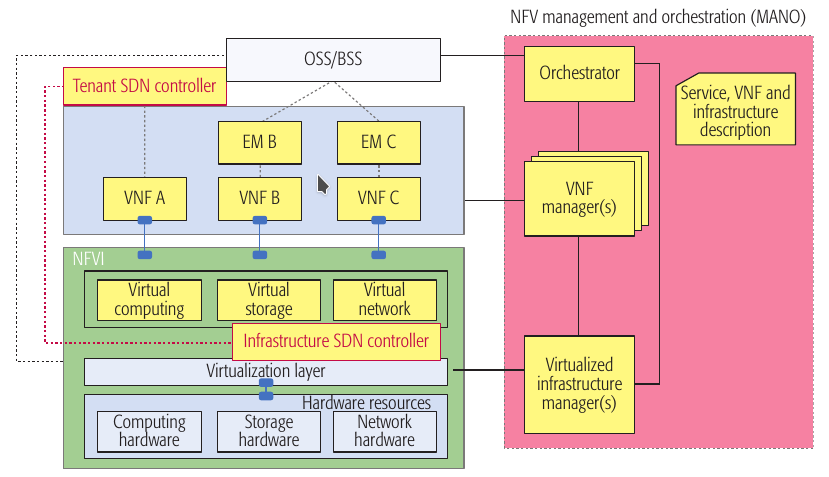
\includegraphics[scale=0.56]{pics/integral.png} 
\caption{Integrating SDN controllers into the reference NFV architectural framework. \cite{ordonez2017network}}
\label{integral}
\end{figure}
\cite{ordonez2017network} \cite{etsi2017gs}


\newpage
\section{Network Slicing} 
Now we have all the players to look inside what NGMN has proposed as the concept of network slicing. The previous telecommunication generation hosted different services as mobile broadband, voice and SMS over the same network architecture, 5G networks will allow shared and customized logical architectures to fulfill the requirements of vertical services as \gls{eMBB}, vehicular communications, \gls{URLLC}, and \gls{mMTC}. These services request different KPIs hardly fulfilled by 3G-4G systems because they are characterized by  network elements with strongly coupled at level of hardware, software, and functionalities. \\
As we previously said, 5G architectures must work on the decoupling of software‐based NFs from the above infrastructure resources by
means of various resource abstraction technologies. Then, exploiting modularization, some resource sharing technologies the actions of multiplexing and multitasking in general which actual example are 
wavelength division multiplexing or radio scheduling, can be supported by NFV and SDN
in software manner techniques to share the not virtualized physical infrastructure.
\begin{figure}[H]
\centering
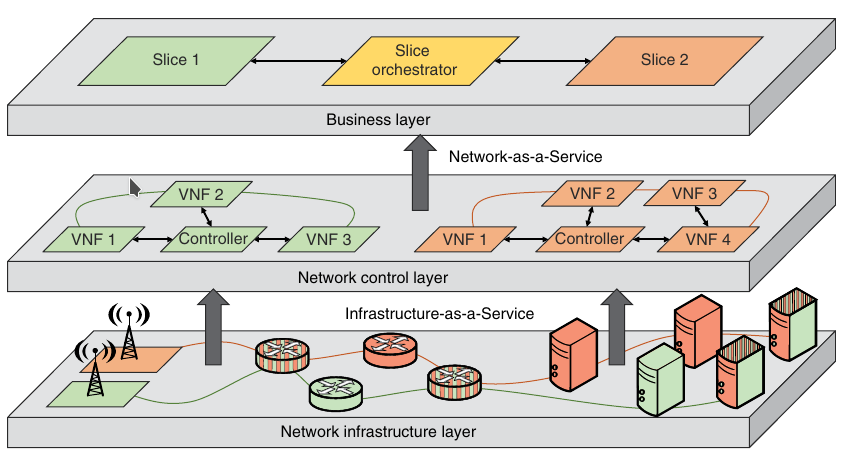
\includegraphics[scale=0.55]{pics/slice.png}
\caption{An example of a network‐sliced architecture. \cite{al20185g}} 
\label{slice}
\end{figure}
Completely decoupled E2E networks can be built over a common and shared infrastructure and in turn multiplexing will not be at infrastructure level (and not anymore at network level), as depicted in Fig. \ref{slice}, carrying out better \gls{QoS} or \gls{QoE} because slices with different peculiarities will be customized for specific services.\\
The concept of network slice says that it is a logical network providing tailored network characteristics and including NFs, enhanced computing and networking resources to fulfill the
KPIs the tenants ask. This involves \gls{RAN} and CN NFs that can include MANO components depending on the degree of freedom a tenant wants to achieve. Thanks to isolation, network slice can be offered to a
single tenant or shared by multiple tenants having same requirements
but different policies or security settings. \\
The hardware/software decoupling allows an efficient slice scaling easing the
economic feasibility of this architecture because it can be dynamically and smartly adapted to demanded resources.\\
The 5G atom proposed in Fig. \ref{atom} summarizes the discussion: in the middle the possible use cases; from the center outwards the layers list the requirements for the cases, the enabling concepts for
operators to get the requirements and the technologies to implement them. \cite{al20185g} \cite{5GPPP}
\begin{figure}[h]
\centering
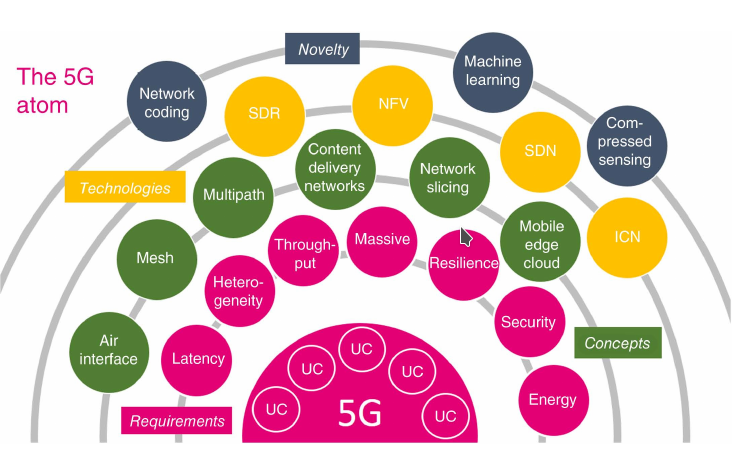
\includegraphics[scale=0.63]{pics/5g_atom.png} 
\caption{5G atom representation. \cite{marsch20185g}}
\label{atom}
\end{figure}


\subsection{Main Services Types}
The three 5G services considered for the beginning are:
\begin{itemize}
\item Enhanced mobile broadband (eMBB): it actually is an evolution of the today 4G network and it is related to operation done by humans with the target to enhance access to multimedia, to give services with improved performance with an increasing QoE. It also has to cope oppisite situations, that is a restricted high density user area with huge traffic and poor mobility of users, and also providing wide area coverage where user mobility is medium or high. Moreover 5G aims to furnish complete coverage everywhere with a guaranteed data rate of 50 Mbps;
\end{itemize}
\begin{itemize}
\item Ultra‐reliable and low-latency communications (URLLC): it is necessary where the requirements for latency and reliability are very strict. It will play a fundamental role in the industry 4.0 and indeed involves situation as remote medical surgery, automation industries and smart grids.
\end{itemize}
\begin{itemize}
\item Massive machine‐type communications (mMTC): it is the realization an efficient Internet of Things, a huge number of devices are connected transmitting a low volume of data traffic, usually non sensitive of the delay which can be about seconds or hours. In general, this devices must be
low-cost with a long lifetime. Some examples are logistics applications, smart metering and agriculture where a lot of sensors are spread around to collect data.
\end{itemize}
Their 8 most important KPIs are the following:
\begin{itemize}
\item Peak data rate: ideal maximum e data rate achievabl per user in bits per second. The minimum requirement is 20 Gbps in downlink and 10 Gbps in uplink;
\end{itemize}
\begin{itemize}
\item User experienced data rate, achievable data rate available on whole coverage area perceived by a mobile user in bits per second. It can be seen as minimum user experience and is set to
100 Mbps in downlink and 50 Mbps in uplink;
\end{itemize}
\begin{itemize}
\item Average spectral efficiency, also called spectrum efficiency, it is the average data
throughput per unit of spectrum resource and per cell in bps/Hz/cell. Here, the minimum requirement depends on the environment:
\begin{itemize}
\item Indoor Hotspot: 9 bps/Hz/cell in downlink, 6.75 bps/Hz/cell in uplink;
\end{itemize}
\begin{itemize}
\item Dense Urban: 7.8 bps/Hz/cell in downlink, 5.4 bps/Hz/cell in uplink;
\end{itemize}
\begin{itemize}
\item Rural: 3.3 bps/Hz/cell in downlink, 1.6 bps/Hz/cell in uplink.
\end{itemize}
\end{itemize}
\begin{itemize}
\item Area traffic capacity, only for indoor,it is the total traffic throughput per area in Mbps/m$^2$, defined only, aiming of 10 Mbps/m$^2$ for downlink;
\end{itemize}
\begin{itemize}
\item User plane latency, time from when the
source have sent a packet to the destination receives it, it is set to 4 ms for eMBB and 1 ms for URLLC;
\end{itemize}
\begin{itemize}
\item Connection density, it is the total number of connected UEs 
per unit area, it targets 1 billion devices per km$^2$ for mMTC;
\end{itemize}
\begin{itemize}
\item Energy efficiency, it is the ratio between users bits transmitted/received and energy consumption of the RAN/device to do the job in bits/Joule.
\end{itemize}
\begin{itemize}
\item Mobility, it is the maximum speed at which a defined QoS is guaranteed while UEs is moving between radio nodes. In rural environment, the normalized traffic channel link data rate is 500 km/h.
\end{itemize}
The following web-spider diagrams in Fig. \ref{cap1}-\ref{cap2}, sum up optimally these capabilities and how they have to be split to realize each particular slice. \cite{marsch20185g} \cite{etsi2018gs} \cite{idc} \cite{al20185g}
\begin{figure}[h]
\centering
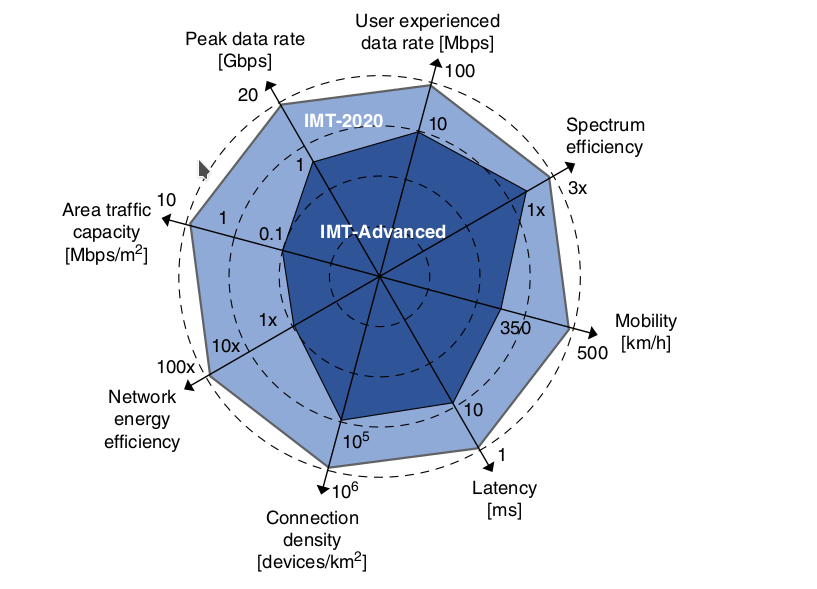
\includegraphics[scale=0.4]{pics/capabilities1.png}
\caption{Capabilities to be achieved. \cite{al20185g}} 
\label{cap1}
\end{figure}
\begin{figure}[H]
\centering
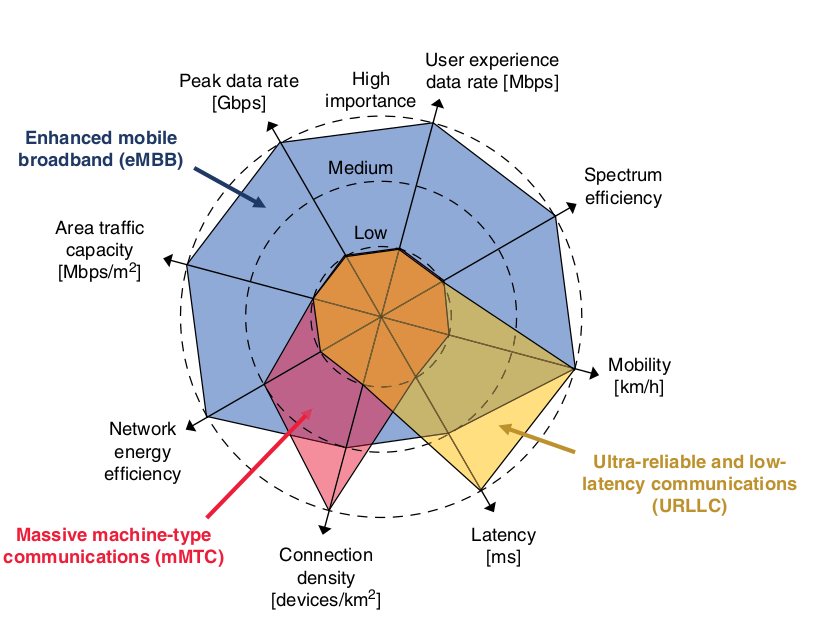
\includegraphics[scale=0.4]{pics/capabilities2.png}
\caption{How capabilities are divided for each slice. \cite{al20185g}} 
\label{cap2}
\end{figure}




\newpage
\section{5G Architecture}
3GPP has decided to release 5G specifications into
two phases, the Release-15 on August 2018 addressing related to commercial
needs and Release-16 is planned for March
2020 to identify all use cases and related requirements. 
Now, a representation of 5G architecture is shown in order to understand how netowork slicing is implemented; Fig. \ref{archite}
\begin{figure}[h]
\centering
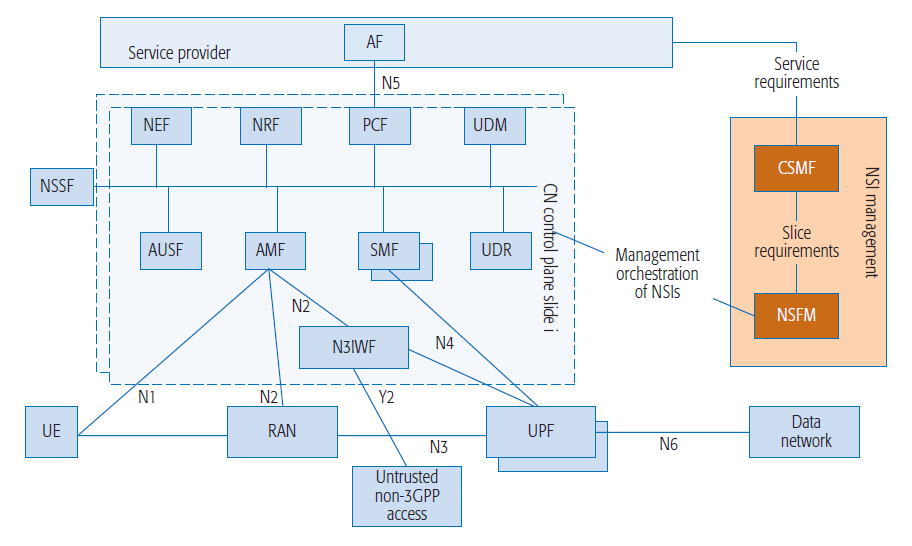
\includegraphics[scale=.57]{pics/5g_architecture.PNG}
\caption{5G System architecture. \cite{etsi2018gs} \cite{kaloxylos2018survey}}
\label{archite}
\end{figure}
The CN is modularized and slice NFs areallocated within it. The CP functions are:
\begin{itemize}
\item Core access and mobility management function
(AMF) necessary to manage mobility, to
authenticate and give authorization, for what concerns security
functions and context selection;

\item Session management function (SMF) handles session
management, allocation of IP addresses, selection of UP functions and QoS;

\item \gls{PCF} gives an unified policy framework to govern network behavior and plane functions;

\item \gls{NEF} makes secure the exposition of the services provided by NFs;

\item \gls{NRF} is a service discovery function exploited by NFs;

\item Unified data management (UDM) involves the repository where the authentication
credentials are stored and the subscription management;

\item Authentication server function (AUSF) supports the authentication server;

\item \gls{N3IWF} is necessary to support non-3GPP access networks;

\item \gls{UDR} stores subscription and policy data;
\end{itemize}
The architecture also contains the following
functions:
\begin{itemize}
\item User plane function (UPF) is an anchor point for mobility, it is mandatory for packet routing and forwarding and define QoS for the UP;

\item \gls{NSSF} necessary to tie UE to a
specific slice;

\item \gls{AF} influences traffic routing, accesses the NEF, interacts with PCF;
\end{itemize}
5G allows UEs to access multiple slices at the same time, but an only AMF will be involved for all slices; 8 slices in parallel is the limit.
To recognize the slices, the network slice selection assistance information and the slice differentiator are exploited; the former is a slice/service type, necessary to recognize the NFs contained in a slice, and the latter is used to distinguish among multiple slices of the same type. 3GPP has
standardized slice/service type values for eMBB, for URLLC and for mMTC. Therefore, CN
is responsible to authorize the attachment of UE
to a slice.\\
The management functions are called \gls{CSMF} and \gls{NSMF}. The first translates the service requirements for communication
to network slice requirements: we are talking about capacity,
throughput, delay, number of users, etc.. The
second takes care of the life cycle of a slice. In general it
consists of the phases:
\begin{itemize}
\item Preparation phase;

\item Instantiation, configuration, and activation
phase;

\item Runtime phase;

\item Decommissioning phase;

\end{itemize}
The first phase is related to the creation of a slice template. During the second phase,
all NFs and resources are allocated and set up. During the third 
a network slice is operating its functions. The last phase concerns the deactivation of a slice and the deallocation of the resources. \cite{kaloxylos2018survey} \cite{etsi2018gs}


\section{Conclusion}
In this work has been given a general and as complete as possible overview of the novel technology of network slicing, starting from necessary concepts and the techniques to implement them arriving to the description of their functions and their requirements defined by ETSI. Then it has been investigated how the network slicing will be inserted in the future 5G architecture.

\phantomsection 
\addcontentsline{toc}{chapter}{Bibliography} 

\newpage
\nocite*
\bibliographystyle{plain}
\bibliography{biblist}

\end{document}